\begin{frame}{Sammensat kvadraturregel}
Trapez-reglen er som sagt, som følger
    \begin{align*}
    T = \frac{h}{2}(f(a)+f(b)),
    \end{align*}
\begin{center}
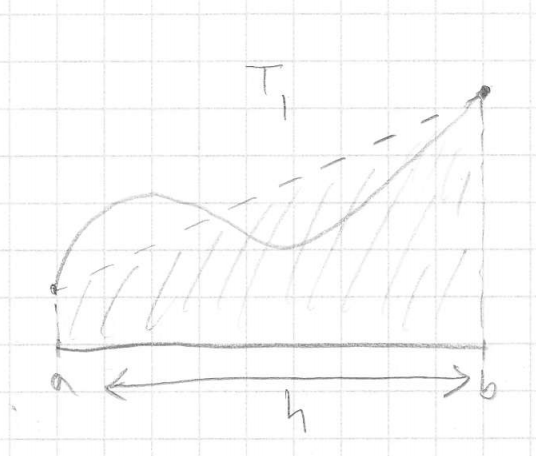
\includegraphics[scale=0.4]{images/TRAPEZZI.png}
\end{center}
\end{frame}

\begin{frame}{Sammensat kvadraturregel}
Man tager sit interval fra a til b og inddeler i ækvidistante inddelinger, hvor $x_0$ angiver a, og $x_n$ angiver b og så gælder der ydermere følgende
    \begin{align*}
    a = x_0 < x_1 < … x_{n-1} < x_n = b
    \end{align*}
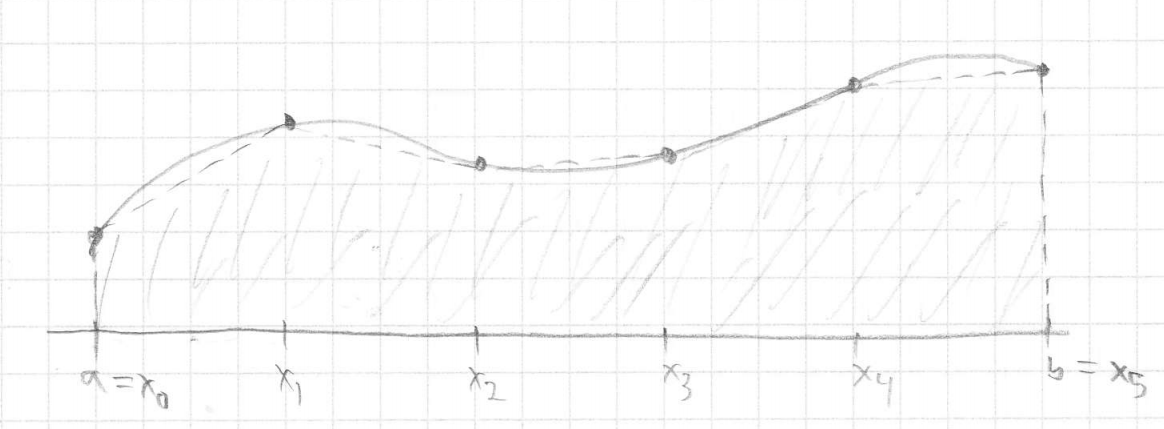
\includegraphics[scale=0.3]{images/TRAPEZSAM.png}
\end{frame}

\begin{frame}{Sammensat kvadraturregel}
    For at udlede trapez-reglen, så den gælder for to underinddelinger, så får man følgende 
    \begin{align*}
    T_2=\frac{h}{2}(f(a)+f(a+h))+\frac{h}{2}(f(a+h)+f(b) \\
    = \frac{h}{2}(f(a)+2f(a+h)+f(b),
    \end{align*}
\begin{center}
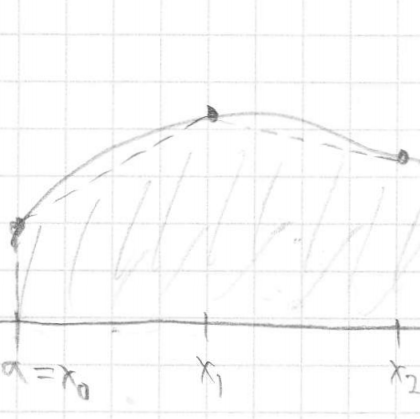
\includegraphics[width=50mm]{images/TRAPEZ12.png}
\end{center}
\end{frame}


\begin{frame}{Sammensat kvadraturregel}
Dernæst er det videre muligt, at opskrive den generelle formel for den sammensatte kvadraturregel $T_n$ givet ved
    \begin{align*}
    T_n = \frac{1}{2}\left (  h\sum_{k=0}^{N-1}f(a+kh)+h\sum_{k=1}^{N}f(a+kh)\right )
    \end{align*}
    som kan reduceres og omskrives til 
    \begin{align*}
    T_n =\frac{h}{2}\left ((f(a)+2\sum_{k=1}^{N-1}f(a+kh)+f(b) \right )
    \end{align*}
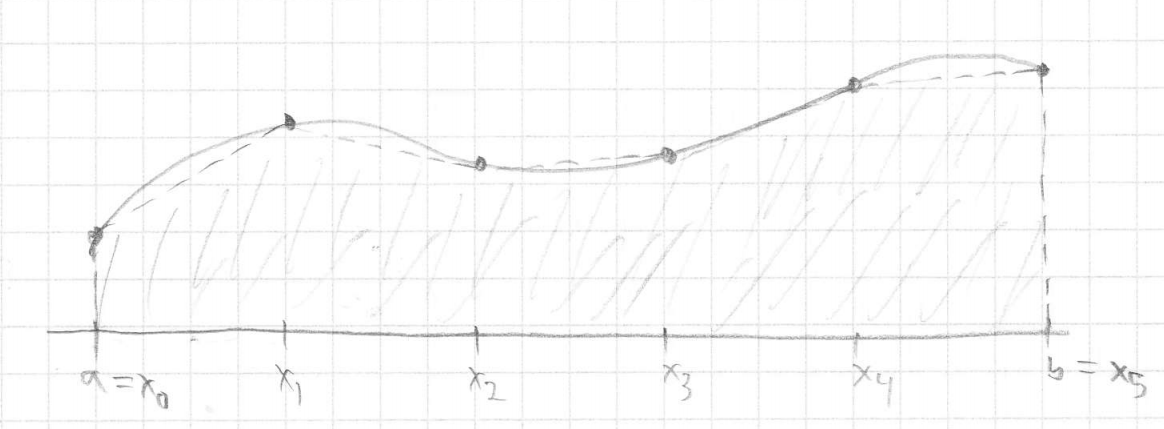
\includegraphics[scale=0.3]{images/TRAPEZSAM.png}
\end{frame}

%%%%